\documentclass{beamer}
\usepackage{wasysym}

\usepackage[framemethod=tikz]{mdframed}
\usepackage[makeroom]{cancel}
\usepackage{tikz}


\setbeamercolor{background canvas}{bg=white}

\tikzstyle{every picture}+=[remember picture]
\usetikzlibrary{arrows,positioning}
\tikzset{
	%Define standard arrow tip
	>=stealth',
	%Define style for boxes
	punkt/.style={
		rectangle,
		rounded corners,
		draw=black, very thick,
		text width=6.5em,
		minimum height=2em,
		text centered},
	% Define arrow style
	pil/.style={
		->,
		thick,
		shorten <=2pt,
		shorten >=2pt,}
}
\usetikzlibrary{positioning}

\usetheme[sectionpage=none,numbering=counter]{metropolis}
%\setbeamertemplate{footline}[frame number]
\usepackage{graphicx}
\usepackage[utf8]{inputenc}
\usepackage[T1]{fontenc} 
\newcommand{\textoverscript}[1]{$^{\text{#1}}$}
\newcommand{\textunderscript}[1]{$_{\text{#1}}$}
\usepackage{caption}
\captionsetup{justification=raggedright,singlelinecheck=false}
\captionsetup[figure]{labelformat=empty}


\setbeamercovered{transparent}% Dim out "inactive" elements
\setbeamertemplate{caption}{\raggedright\insertcaption\par}
\setlength\abovecaptionskip{-15pt}
\newcommand{\tabitem}{%
  \usebeamertemplate{itemize item}\hspace*{\labelsep}}
\title{Velocity Distribution Functions of Pickup Ions with Ulysses/SWICS}
\subtitle{Master Thesis Results}
%\subtitle{MNF-phys-1321 -- Methodenkenntnisse und Projektplanung}
\author{Anne Fischer}
\date{\today}
%
%
%
\begin{document}

%%%
\begin{frame}{Data from the ULYSSES FINAL ARCHIVE}
\begin{figure}									
	\includegraphics[width=1.05\textwidth]{Pics/data_files.png}
\end{figure}

\end{frame}

%%%
\begin{frame}{Coordinate Systems}
\begin{figure}									
	\includegraphics[width=.9\textwidth]{Pics/HELIO_coordsystems.png}
\end{figure}

\end{frame}

%%%
\begin{frame}{Ulysses' 1st Orbit}
\begin{columns}
	\begin{column}{0.5\textwidth}
		\begin{figure}
			\hspace{-.7cm}									
			\includegraphics[width=1.1\textwidth]{Pics/ulysses_trajectory.pdf}
		\end{figure}
	\end{column}

	\begin{column}{0.5\textwidth}
		\vspace{-.5cm}
		\includegraphics[width=1.15\textwidth]{Pics/ECL_LAT.png}
		\vspace{-.5cm}
		\includegraphics[width=1.15\textwidth]{Pics/ECL_LONG.png}
	\end{column}
\end{columns}

\end{frame}
%%%
\begin{frame}{Ecliptic System -- Latitude}
%\vspace{-.8cm}
\begin{figure}									
	\includegraphics[width=1.0\textwidth]{Pics/ECL_LAT_zoom.png}
\end{figure}
\end{frame}

%%%
\begin{frame}{Ecliptic System -- Latitude}
%\vspace{-.8cm}
\begin{figure}									
	\includegraphics[width=1.0\textwidth]{Pics/ECL_LAT_zoom_rou.png}
\end{figure}
\end{frame}

%%%
\begin{frame}{Ecliptic System -- Latitude}
%\vspace{-.8cm}
\begin{figure}									
	\includegraphics[width=1.0\textwidth]{Pics/ECL_LAT_diff.png}
\end{figure}
\end{frame}

%%%
\begin{frame}{Ecliptic System -- Longitude}
%\vspace{-.8cm}
\begin{figure}									
	\includegraphics[width=1.0\textwidth]{Pics/ECL_LONG_diff.png}
\end{figure}
\end{frame}


\begin{frame}{Equatorial System}
%\vspace{-.8cm}
\begin{figure}									
	\includegraphics[width=.7\textwidth]{Pics/KrystynaRef.png}
\end{figure}
\end{frame}



\begin{frame}{Equatorial System -- Latitude}
\begin{figure}									
	\includegraphics[width=1\textwidth]{Pics/EQ_LAT.png}
\end{figure}
\end{frame}

\begin{frame}{Equatorial System -- Longitude}
\begin{figure}									
	\includegraphics[width=1\textwidth]{Pics/EQ_LONG.png}
\end{figure}
\end{frame}

\begin{frame}{Equatorial System -- Latitude calculated}
\begin{figure}									
	\includegraphics[width=1\textwidth]{Pics/EQ_LAT_CALC.png}
\end{figure}
\end{frame}

\begin{frame}{Equatorial System -- Longitude calculated}
\begin{figure}									
	\includegraphics[width=1\textwidth]{Pics/EQ_LONG_CALC.png}
\end{figure}
\end{frame}

\begin{frame}{Equatorial System -- Longitude -- B1950 vs. J2000}
\begin{figure}									
	\includegraphics[width=1\textwidth]{Pics/EQ_LONG_J_B.png}
\end{figure}
\end{frame}

\begin{frame}{Equatorial System -- Latitude --  B1950 vs. J2000}
\begin{figure}									
	\includegraphics[width=1\textwidth]{Pics/EQ_LAT_J_B.png}
\end{figure}
\end{frame}

\begin{frame}{Aspect Angle}
\begin{columns}
	\column[]{6.cm}
			\vspace{-2.8cm}
		\begin{figure}
			\includegraphics[scale=0.4]{Pics/RTN_AA_angles.pdf}
		\end{figure}
		\vspace{2cm}
	\column[]{1cm}
	\column[]{6cm}
		\vspace{1.cm}
	\begin{figure}
		\vfill
		\vspace{1.4cm}

		\includegraphics[scale=0.36]{Pics/col_aa_marker.png}
	\end{figure}
\end{columns}
\end{frame}


%%%
\begin{frame}{}
\begin{figure}
	\includegraphics[scale=0.7]{Pics/aa_vergleich_all.png}
\end{figure}
\end{frame}

%%%
\begin{frame}{SPICE Reference Frame Kernel}
\flushleft
\begin{figure}								
	\includegraphics[width=1.1\textwidth]{Pics/kernel_instruction.png}
\end{figure}
\end{frame}




\begin{frame}{}

\end{frame}


%
%
\end{document}